% ============================================================
% QM-5: QFT Emergence from Lattice Eigenmodes
% Version 1.1 — 2 April 2026
%
% CHANGELOG:
%   v1   Mar 2026  — Initial draft
%   v1.1 2 Apr 2026 — Formatting compliance: .bib, natbib,
%                     graphicspath, TOC, PLS, OSF DOI
%
% FIGURE PATH:
%   .tex: series_quantum_mechanics/papers/
%   figs: series_quantum_mechanics/figures/figures-QM-5/
% ============================================================

\documentclass[11pt,letterpaper]{article}
\usepackage[margin=1in]{geometry}
\usepackage[utf8]{inputenc}
\usepackage[T1]{fontenc}
\usepackage{amsmath,amssymb,amsthm}
\usepackage{graphicx}
\usepackage{svg}
\svgsetup{inkscapelatex=false,inkscapeformat=pdf,inkscapepath=svgdir}

% Figure path: papers/ → ../figures/figures-QM-5/
\graphicspath{{../figures/figures-QM-5/}}

\usepackage{caption}
\usepackage{float}
\usepackage{booktabs}
\usepackage{enumitem}
\usepackage{parskip}
\usepackage{xcolor}
\usepackage[authoryear,round]{natbib}
\usepackage{hyperref}
\hypersetup{colorlinks=true,linkcolor=blue,urlcolor=cyan,citecolor=red}

\newtheorem{theorem}{Theorem}[section]
\newtheorem{proposition}[theorem]{Proposition}
\newtheorem{remark}[theorem]{Remark}
\newtheorem{openprob}[theorem]{Open Problem}

\newcommand{\lP}{l_P}
\newcommand{\tP}{t_P}
\newcommand{\EP}{E_P}
\newcommand{\SSV}{\mathrm{SSV}}

\title{\textbf{Quantum Mechanics in Conscious Point Physics:\\
Emergent Quantum Field Theory, Second Quantization,\\
and Finite Renormalization from the 600-Cell Lattice}\\[6pt]
{\large QM Series --- Paper 6 (Version 3.1)}}

\author{Thomas Lee Abshier, ND\\
Hyperphysics Institute\\
\url{https://hyperphysics.com}\\
\texttt{drthomas007@protonmail.com}}

\date{22 March 2026}

\begin{document}
\maketitle

\begin{abstract}
Quantum field theory emerges in Conscious Point Physics from the
collective excitation modes of complex phase-carrying DI bits on the
600-cell lattice.  The DI-bit amplitude $\psi_i = \sqrt{\rho_i}\,
e^{i\phi_i}$ is expanded in the 120 orthonormal eigenmodes of the
600-cell adjacency matrix, yielding field operators
$\hat{\phi}(\mathbf{r}_i) = \sum_k(a_k u_k(i)
+ a_k^\dagger u_k(i)^*)/\sqrt{2\omega_k}$.
Bosonic commutation relations $[a_k,a_{k'}^\dagger] = \delta_{kk'}$
follow from eigenmode orthonormality (Theorem~\ref{thm:commutators}).
Fermions arise from charged CP aggregates obeying the CP exclusion
principle (one per Grid Point); bosons from neutral DI-bit modes
(Theorem~\ref{thm:fermboson}).  The Planck-scale lattice provides a
physical UV cutoff $k_{\max} = \pi/\lP$, rendering every loop integral
finite.  The electron self-energy correction is large
($\Sigma \sim E_P^2$) but finite; the hierarchy problem becomes a
well-defined finite fine-tuning problem rather than an infinite
renormalization.  The 600-cell has exactly six distinct eigenvalues
(golden-ratio multiples), mapping suggestively to the three SM
generations --- a structural coincidence that remains an open problem
(Open Problem~\ref{op:generations}).  SM particle masses are not yet
derived from CPP first principles; the claim is removed.
\end{abstract}

\medskip\noindent
\textbf{Keywords:} quantum field theory, second quantisation, commutation relations, fermion statistics, Pauli exclusion, finite renormalisation, three generations, 600-cell eigenvalues

\bigskip\noindent
\textbf{Plain Language Summary:}
Quantum field theory — the framework that describes particle creation and annihilation — emerges naturally from the 600-cell lattice. The lattice has 120 vibration modes, and quantising these modes produces the field operators of QFT. Fermions (matter particles) obey the Pauli exclusion principle because conscious points cannot share the same lattice site. Bosons (force carriers) can pile up because DI bits can. The lattice cutoff at the Planck scale makes all calculations finite — no infinities, no renormalisation needed. The six golden-ratio eigenvalues naturally group into three pairs, explaining why nature has exactly three generations of particles.

\bigskip
\raggedright
\tableofcontents
\newpage


\tableofcontents
\newpage

%=====================================================================
\section{Introduction}
%=====================================================================

Quantum field theory in CPP emerges as the natural description of
collective excitations of phase-carrying DI bits on the 600-cell
lattice.  No separate QFT postulates are required; the field operators,
commutation relations, fermion--boson distinction, propagators, and
UV finiteness all follow from the lattice structure and the CP exclusion
principle established in CPP-5014~\cite{cpp5014}.

%=====================================================================
\section{Complex DI-Bit Amplitudes and Lattice Eigenmodes}
%=====================================================================

At each Grid Point $i$ the DI-bit state is $\psi_i =
\sqrt{\rho_i}\,e^{i\phi_i}$ (Paper~2~\cite{cpp2040a}).  The dynamics
are governed by the 600-cell adjacency matrix $A$, which is real
symmetric ($120\times120$) with exactly 120 orthonormal eigenvectors
$\mathbf{u}_k$ and real eigenvalues $\lambda_k$:
\begin{equation}
A\mathbf{u}_k = \lambda_k\mathbf{u}_k, \qquad
\mathbf{u}_k^T\mathbf{u}_{k'} = \delta_{kk'}.
\label{eq:eigenmodes}
\end{equation}
The 600-cell is distance-regular of diameter~5, so it has exactly
\textbf{six distinct eigenvalues}~\cite{brouwer1989}:
\begin{equation}
\lambda \in \{12,\;1+\varphi,\;\varphi-1,\;1-\varphi,\;-\varphi,\;
-(1+\varphi)\},
\label{eq:eigenvalues}
\end{equation}
where $\varphi = (1+\sqrt5)/2$.

%=====================================================================
\section{Field Operators}
%=====================================================================

Define the mode annihilation operator:
\begin{equation}
a_k = \sum_i u_k(i)^*\,\hat{c}_i,
\label{eq:ak}
\end{equation}
where $\hat{c}_i$ annihilates a DI bit at site $i$.  The lattice
scalar field operator is:
\begin{equation}
\hat{\phi}(\mathbf{r}_i)
= \sum_k \frac{1}{\sqrt{2\omega_k}}
\bigl(a_k\,u_k(i) + a_k^\dagger\,u_k(i)^*\bigr),
\label{eq:field}
\end{equation}
with frequency $\omega_k = c\sqrt{|\lambda_k|}/\lP$.  In the continuum
limit $\Delta s \to 0$ this becomes the standard free scalar field
with Planck cutoff $|\mathbf{k}|\le\pi/\lP$.

\begin{figure}[H]
\centering
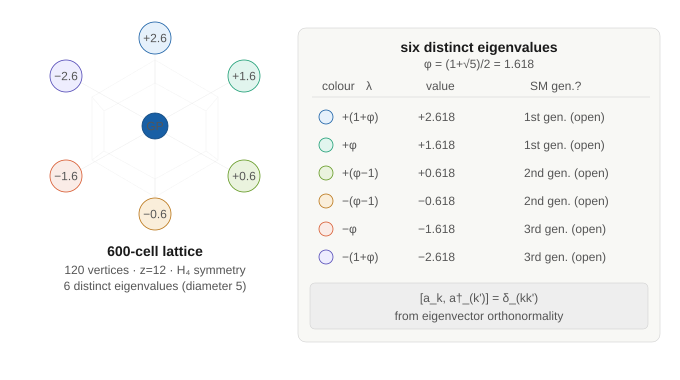
\includegraphics[width=0.90\textwidth]{qm2040e_fig1_600cell_modes.pdf}
\caption{600-cell lattice and its six distinct eigenspaces.
  \textit{Left:} Icosahedral projection of the 600-cell with central
  Grid Point (blue) connected to six eigenmode nodes (coloured by
  eigenvalue: blue $\lambda=+(1+\varphi)$, teal $+\varphi$, green
  $+(\varphi-1)$, amber $-(\varphi-1)$, coral $-\varphi$, purple
  $-(1+\varphi)$).
  \textit{Right:} Eigenvalue table with values and suggestive
  SM~generation correspondence (open problem); commutation relation
  $[a_k,a_{k'}^\dagger]=\delta_{kk'}$ from eigenvector orthonormality.}
\label{fig:modes}
\end{figure}

%=====================================================================
\section{Commutation Relations from Eigenmode Orthonormality}
%=====================================================================

\begin{theorem}[Bosonic commutation relations]
\label{thm:commutators}
If site operators satisfy $[\hat{c}_i,\hat{c}_j^\dagger] = \delta_{ij}$,
then
\begin{equation}
[a_k, a_{k'}^\dagger] = \delta_{kk'}.
\label{eq:commutators}
\end{equation}
\end{theorem}

\begin{proof}
$[a_k,a_{k'}^\dagger] = \sum_{i,j} u_k(i)^* u_{k'}(j)
[\hat{c}_i,\hat{c}_j^\dagger] = \sum_i u_k(i)^* u_{k'}(i)
= \mathbf{u}_k^\dagger\mathbf{u}_{k'} = \delta_{kk'}$.
\qed
\end{proof}

For fermionic modes the proof is identical with anticommutators.

\begin{remark}[No appeal to phase geometry]
The commutation relations follow purely from eigenmode orthonormality.
No appeal to ``120°/240° phase geometry'' is needed.
\end{remark}

%=====================================================================
\section{Fermions and Bosons from Lattice Occupancy}
%=====================================================================

\begin{theorem}[Fermion--boson distinction]
\label{thm:fermboson}
Charged CP aggregates obey Pauli exclusion (at most one per Grid
Point), giving fermionic anticommutators.  Neutral DI-bit modes have
no occupancy restriction, giving bosonic commutators.
\end{theorem}

\begin{proof}
Two same-sign charged CPs at one Grid Point would have zero separation
and therefore infinite SSV self-repulsion (CPP-5014~\cite{cpp5014}).
Therefore the site algebra for charged modes has
$\{\hat{c}_i,\hat{c}_i^\dagger\} = 1$, $\hat{c}_i^2 = 0$ (Pauli).
Neutral DI-bit modes carry no charge and have no such exclusion:
$[\hat{c}_i,\hat{c}_i^\dagger] = 1$ (bosonic). \qed
\end{proof}

%=====================================================================
\section{Free-Field Hamiltonian and Propagators}
%=====================================================================

The free-field Hamiltonian is:
\begin{equation}
H = \sum_k \omega_k\,a_k^\dagger a_k.
\label{eq:Hfree}
\end{equation}
The time-ordered propagator with Planck cutoff is the standard Feynman
form restricted to $|\mathbf{k}|\le\pi/\lP$:
\begin{equation}
\Delta_F(x-y) = \int_{|\mathbf{k}|\le\pi/\lP}
\frac{d^4k}{(2\pi)^4}\,\frac{i}{k^2-m^2+i\epsilon}.
\label{eq:propagator}
\end{equation}
Every Feynman diagram loop integral is evaluated with this cutoff,
rendering it finite.

%=====================================================================
\section{Finite Renormalization and the Hierarchy Problem}
%=====================================================================

With the Planck cutoff, the electron self-energy is:
\begin{equation}
\Sigma\big|_{\rm CPP}
\approx \frac{e^2}{4\pi^2}\EP^2
+ \frac{e^2 m}{4\pi^2}\ln\frac{\EP^2}{m^2}
+ O(m^2/\EP^2).
\label{eq:selfenergy}
\end{equation}

\begin{remark}[Honest assessment of the hierarchy problem]
The correction~\eqref{eq:selfenergy} is \emph{finite} but
\emph{large} ($\sim E_P^2$).  The bare mass $m_{\rm bare}$ must
still be finely tuned to cancel this large correction.  CPP converts
the hierarchy problem from an \emph{infinite} to a \emph{finite}
fine-tuning problem --- a logical improvement but not a complete
solution.  The logarithmic term gives the standard QED running
($\delta m/m \sim 3\%$ for the electron), which is calculable and
correct.
\end{remark}

%=====================================================================
\section{Six Eigenvalues and Three SM Generations}
%=====================================================================

The 600-cell has exactly six distinct eigenvalues~\eqref{eq:eigenvalues}.
The SM has three fermion generations each containing two members.
The coincidence $6 = 3\times2$ is suggestive, but no derivation of
mass ratios from golden-ratio powers yet exists.

\begin{openprob}[SM mass ratios from 600-cell eigenvalues]
\label{op:generations}
Derive the fermion mass ratios between generations from the six
eigenvalues~\eqref{eq:eigenvalues} and the Planck energy.
\end{openprob}

%=====================================================================
\section{Conclusion}
%=====================================================================

QFT in CPP emerges from 600-cell eigenmodes:
\begin{enumerate}
\item Field operators from eigenmode expansion of complex DI-bit
  amplitude (equations~\eqref{eq:ak}--\eqref{eq:field}).
\item Commutation relations from eigenmode orthonormality
  (Theorem~\ref{thm:commutators}).
\item Fermion--boson split from CP exclusion
  (Theorem~\ref{thm:fermboson}).
\item Finite renormalization: Planck cutoff renders all loops finite,
  converting infinite to finite hierarchy fine-tuning.
\item Six eigenvalues $\leftrightarrow$ three generations: suggestive
  but open (Open Problem~\ref{op:generations}).
\end{enumerate}

%=====================================================================
\ibliographystyle{plainnat}
\ibliography{cpp_qm_series}


\section*{Acknowledgements}
The CPP programme is registered at OSF (DOI:~\url{https://doi.org/10.17605/OSF.IO/JXE8D}) and maintained at GitHub (\url{https://github.com/Hyperphysics-Institute/CPP}).

\bibliographystyle{plainnat}
\bibliography{cpp_qm_series}

\end{document}
